\clearpage
\chapter{\textbf{Lokalisierung - Lösungsansätze}}\label{chap:Lokalisierung - Lösungsansätze}
\addtocontents{toc}{\vspace{0.8cm}}
Das Themengebiet der Lokalisierung in der mobilen Robotik ist ein Grundstein für die Funktionalität dieser. Ohne Informationen über den genauen Standort könnte ein Räsenmäherroboter den Garten nicht schön halten, ein nach einem Paket greifenden UAV das Ziel nicht treffen oder eine Handvoll Fußball spielender Roboter den Ball nicht treffen. Dabei sind drei verschiedene Arten der Lokalisierung ausschlaggebend: Die \textit{Global Localization}, das \textit{Position Tracking} und die \textit{Kidnapping Recovery}. Die globale Lokalisierung beschreibt die Fähigkeit des Systems die korrekte erste Position in einer gegebenen Karte zu bestimmen. Das Position Tracking befasst sich mit der Aufgabe eine gefundene Position bei Bewegung des Systems beizubehalten, während die Kidnapping Recovery die Herausforderung beschreibt den Standort des mobilen Roboters nach einem Entführungsszenario wiederherzustellen. Ein Entführungsszenario meint hierbei das Bewegen des Systems, ohne dass die externen, Umgebung erfassenden Sensoren aktiv sind. In den folgenden Kapiteln werden ein paar Lösungsansätze und ausformulierte Algorithmen zur Lösung des Lokalisierungsproblems vorgestellt.

\section{Monte Carlo Localization}\label{sec:mcl}
\addtocontents{toc}{\vspace{0.8cm}}
Der von Daeller et al. \cite{Monte-Carlo-Localization} entwickelte \textit{Monte Carlo Localization} (MCL) Lokalisierungsalgorithmus verfolgt das Ziel einen mobilen Roboter in bekannter Umgebung zu orten. Der Algorithmus bekommt eine 2D Occupancy Grid Map, das Motion-Model und das Oberservation-Model des Systems zur Verfügung gestellt, generiert damit eine geschätzte 2D Position und ist in der Lage sowohl Position-Tracking, Globale Lokalisierung, als auch Kidnapping-Recovery zu absolvieren. \\
Es handelt sich hierbei um einen Partikelfilter, bei dem jedes Partikel eine mögliche Position des mobilen Systems ohne Toleranz darstellt. Die Einschätzung der Position $Bel(l)$ wird dargestellt durch ein \textit{N}-zahliges Set von gewichteten, zufälligen Partikeln oder \textit{Samples}.Ein Sample kann dargestellt werden durch $s=\langle\langle x,y,\psi \rangle,p\rangle$, wobei die $\langle x,y,\psi$ die Position, und $p$ das Gewicht beziehungsweise die Wahrscheinlichkeit dieser Position repräsentiert. Das Vorgehen ist eingeteilt in die Schritte \textbf{Robot Motion} und \textbf{Sensor readings}. Folglich wird der Algorithmus beginnend mit dem Schritt \textbf{Sensor readings} erläutert.\\
Im Beispiel \ref{fig:mcl} wird die eindimensionale Position eines mobiler Roboter berechnet, indem er auf einer Geraden an mehreren Türen entlang fährt. Ein außen montierter Sensor gibt an, ob er sich an einer Tür befindet. Zum Zeitpunkt der Intialisierung des Algorithmus wird das erste Set an Samples mit vollkommen willkürlichen Positionen, und dem Gewicht $p=N^{-1}$ generiert. Dann folgt der Schritt Sensor readings \ref{fig:s_mcl_sensor} wird das Observation-Model genutzt um die Umgebung wahrzunehmen, und von jedem individuellen Sample aus zu berechnen wie wahrscheinlich die erhaltene Messung an der Position \textit{l} des Samples ist. Die Gewichtungen $p$ der einzelnen Samples in dem Sample-Set werden dann entsprechend der Ergebnisse angepasst, sodass $\sum_{n=1}^{N} p_n =1$ gilt. Je wahrscheinlicher die reale Messung am Ort des Samples ist, desto höher ist dessen Gewichtung.\\
Es folgt der Schritt Robot Motion \ref{fig:s_mcl_motion}: Der Roboter bewegt sich, der Algorithmus generiert ein neues Set mit $N$ neuen Samples, die mithilfe des Motion-Models die neue Position nach der Bewegung annähern. Dafür werden per Zufallsverfahren Samples aus dem vorherigen Set entnommen gegebenenfalls vervielfacht und jedes Gewicht durch $N^{-1}$ ersetzt. Zusätzlich werden dem Set ein wenig neue Samples mit willkürlich generierten Positionen hinzugefügt. Das hilft dem System dabei sich im Falle eines Kidnapping-Szenarios neu zu lokalisieren. Anschließend macht der mobile Roboter wieder Gebrauch von seinem Observation-Model und führt den Schritt Sensor readings wieder aus. Das Partikel mit dem zuletzt höchsten Gewicht stellt die aktuelle Position des Roboters dar. Je mehr Iterationen durchgeführt werden, desto näher befinden sich die Partikel beieinander und desto genauer wird die angenäherte Position.
\mbox{}
\begin{figure}
  \begin{subfigure}[t]{.5\textwidth}
    \centering
    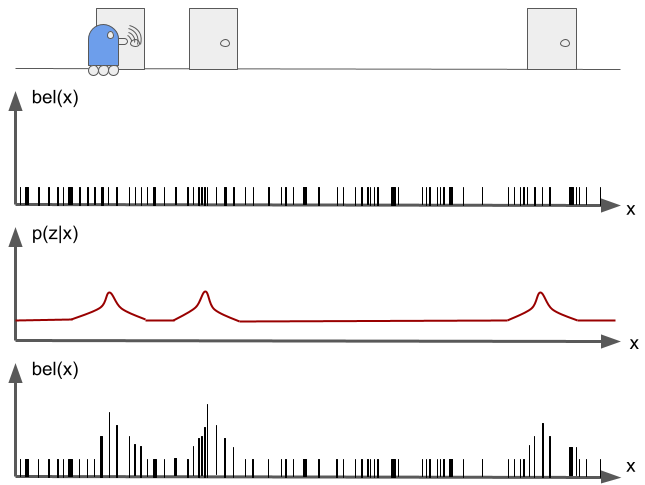
\includegraphics[width=.9\linewidth]{pic/loesungen/1a_mcl.png}
    \caption{Sensor readings}
    \label{fig:s_mcl_sensor}
  \end{subfigure}\hfill
  \begin{subfigure}[t]{.5\textwidth}
    \centering
    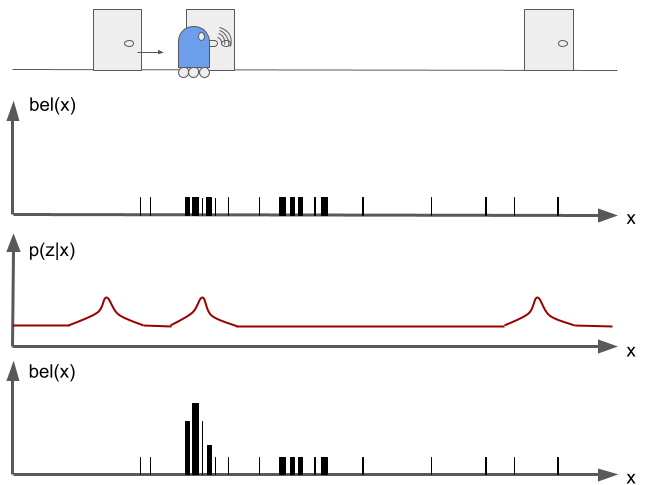
\includegraphics[width=.9\linewidth]{pic/loesungen/1b_mcl.png}
    \caption{Robot Motion}
    \label{fig:s_mcl_motion}
  \end{subfigure}
  \caption{Der MCL Algorithmus aufgeteilt in \textbf{Sensor readings} und \textbf{Robot Motion}}
  \label{fig:mcl}
\end{figure}
\mbox{}


\subsection{Adaptive Monte Carlo Localization}\label{subsec:amcl}
\addtocontents{toc}{\vspace{0.8cm}}
Der Adaptive Monte Carlo Localization (AMCL) Algorithmus ist eine leichte Abwandlung gegenüber des herkömmlichen MCL Algorithmus, der die Größe des Sample-Sets variiert. In MCL ist die Größe des Sample-Sets nach einmaliger Einstellung unveränderbar, dh. es werden für die Berechnung der Position in jeder Iteration die gleiche Menge an Partikeln benutzt. AMCL verfolgt das Ziel einer zumindest gleichwertigen, wenn nicht sogar besseren Positionsbestimmung wie MCL, will dabei aber ressourcenschonender sein. Das erreicht der Algorithmus, indem er die Anzahl der genutzten Partikel abhängig von der Unsicherheit über die errechnete Position dynamisch anpasst.\\
Das Position Tracking benötigt für eine genügend genaue Standortbestimmung wesentlich weniger zu berechnende Partikel, als die weitaus größere Herausforderung der globalen Lokalisierung oder der Kidnapping Recovery. Für die dynamische Festlegung der Größe der Sets wird die Abweichung zwischen dem \textit{belief} vor und nach der Messungen der externen Sensoren berechnet. Je größer hierbei die Überraschung der Sensordaten ist, desto größer wird das nächste Sample-Set gewählt. Der AMCL Algorithmus wird auch heutzutage, trotz seines Alters, in vielen Applikationen verwendet, da es schnell eine Position mit geringem Fehler berechnet.
% TODO Behauptungen hier belegen


\subsection{Monte Carlo Lokalisierung mit Surfel Grid Maps}\label{subsec:mcl_surfel}
\addtocontents{toc}{\vspace{0.8cm}}
\begin{wrapfigure}{R}{0.3\textwidth}
    \centering
    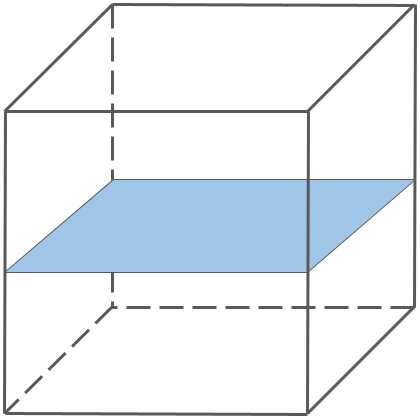
\includegraphics[width=0.28\textwidth]{pic/loesungen/12_surfel.png}
    \caption{Surface Element in a Voxel}
    \label{fig:surfel}
\end{wrapfigure}
Kläß et al. \cite{3DsurfelGridMaps} haben 2012 einen Algorithmus vorgestellt, dessen Ziel eine 2D Positionsbestimmung anhand einer 3D Voxel Grid Map ist. Die Lokalisierung wurde in der Veröffentlichung indoor durchgeführt und soll auch in dynamischen Szenarien, wenn sich beispielsweise bewegende Menschen in der Umgebung befinden, genau funktionieren können.\\
Die Besonderheit dieser Herangehensweise liegt in der Repräsentation der Umgebung. Die Umgebung wird durch eine vielzahl an Voxel (Würfel) modelliert, in denen sich jeweils ein \textit{Surface Element} oder kurz Surfel befindet (siehe bild). Befindet sich bei der Modellierung der Umgebung ein Objekt in einem Voxel, so wird ein Surfel entsprechend der Oberfläche des Objektes im Voxel generiert.\\
Die dahinter liegenden Berechnungen basieren auf MCL. Der Schritt Robot Motion bleibt bestehen, der der Sensor readings wird allerdings den neuen Techniken abgewandelt. Die Autoren schlagen für die verwendeten Sensor Models je nach Bedarf das \textit{Plane-to-Plane Model} oder das \textit{Line-to-Plane Model} vor. Ersteres stellt ein Oberservation-Model speziell für Sensorik, die 3D Scans in der 3D Surfel Grid Map durchführen soll, wie etwa LiDAR vor. Das Line-to-Plane Model hingegen zeigt eine mögliche Implementierung für Sensorik, die 2D Scans in der 3D Surfel Grid Map leisten soll. Aufgrund der fehlenden Dimension kann in letzterem Modell die Orientierung der Normale des Surfels nicht berücksichtigt werden.\\
Das System wurde vor allem in Hinblick auf die Navigation von bodengebundenen mobilen Robotern entwickelt. Das neuartige Surface Element soll dazu dienen die problematischen Diskretisierungseffekete von herkömmlichen 3D Voxel Grid Maps zu verringern (siehe Bild). Außerdem soll die Lokalisierung in dynamischen Szenarien erleichtert werden, indem der Algorithmus sich die 3D Map vollständig zu Nutze macht und sich dann auf Messungen über der Höhe des Menschen konzentriert um eine erfolgreiche Ortung durchzuführen.
% TODO Ergebnisse der Experimente einbringen
\mbox{}
\begin{figure}
  \begin{subfigure}[t]{.5\textwidth}
    \centering
    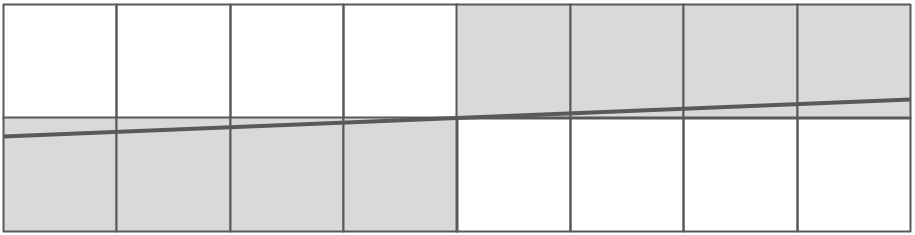
\includegraphics[width=.9\linewidth]{pic/loesungen/12a_steps.png}
    \caption{Generierung von Stufen}
    \label{fig:s_12steps}
  \end{subfigure}\hfill
  \begin{subfigure}[t]{.5\textwidth}
    \centering
    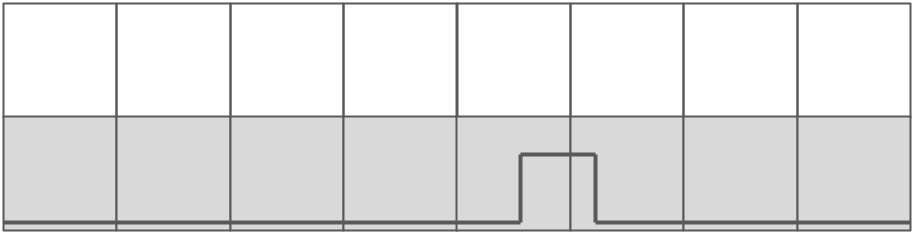
\includegraphics[width=.9\linewidth]{pic/loesungen/12b_bumps.png}
    \caption{}
    \label{fig:s_12bumps}
  \end{subfigure}
  \caption{typische Diskretisierungseffekte in Occupancy Voxel Maps \cite{3DsurfelGridMaps}}
  \label{fig:discretization_effects}
\end{figure}
\mbox{}


\subsection{Dreidimensionale Indoor Lokalisierung}\label{subsec:3d_indoor}
\addtocontents{toc}{\vspace{0.8cm}}
Perez-Grau et al. \cite{dreidimensionale_indoor_lokalisierung} haben 2017 ein System zur dreidimensionalen Positionsbestimmung eines UAV in einem geschlossenen Raum vorgestellt. Der Ansporn zu dessen Entwurf liegt in der industriellen Nutzung von UAVs, wie beispielsweise dem Transportieren von Gegenständen.\\
Die Umgebung wird in Voxeln modelliert und es werden mehrere Sensoren benutzt um mithilfe des MCL Algorithmus eine 3D Position errechnen zu können (siehe Bild \ref{fig:3d_indoor_system}). Eine RGB-D Kamera wird genutzt um sowohl RGB-Bilder, als auch Point Clouds erfassen zu können. Außerdem werden drei sogenannte \textit{ultra-wideband Beacons} (UWB Beacons) genutzt, um per Triangulation einen Standort des UAVs im Raum errechnen zu können. Die Odometry ist hierbei nicht nur von einer IMU abhängig, sondern nutzt ebenfalls die Bilder der Kamera, als auch dessen Point Clouds. So soll eine möglichst genau \textit{Prediction} (Vorhersage) im Robot Motion Schritt des MCL generiert werden, die dann durch ein Update (Sensor readings) berichtigt wird. Diese Berichtigung ist abhängig von den 3D Point Clouds der Kamera, der 3D Voxel Map und den Distanzen zu den drei, im Raum verteilten, UWB Beacons. Die daraus errechnete 3D Position beinhaltet nicht die Nick- und Rollwinkel. Diese werden direkt aus den Berechnungen der IMU entnommen.\\
Der Raum in dem das System getestet wurde ist mit Kameras ausgestattet worden, um den wahren Standort des UAVs, unabhängig vom entworfenen System, erhalten zu können. So konnte ein mehr als 500 Sekunden langer Testflug unternommen werden, bei dem der Fehler der Odometry und der Fehler des MCL genau bestimmt werden konnten (siehe Bild ).
